\documentclass[a4paper,10pt]{article}
\usepackage[a4paper, total={6in, 8in}]{geometry}
\setlength\parindent{0pt}
\usepackage[utf8]{inputenc}
\usepackage{graphicx} 
\usepackage{amsmath}
\usepackage{amsfonts}
\usepackage{amssymb}
\usepackage{listings}
\usepackage{ragged2e}
\usepackage{listings}
\usepackage{color}
\usepackage[table]{xcolor}
\usepackage{soul}
\usepackage[font=small,labelfont=bf]{caption}
\setlength{\parskip}{\baselineskip}%
\setlength{\parindent}{0pt}%

\begin{document}
\begin{titlepage}
	\centering
	
\includegraphics[width=.6\textwidth]{liu-logo.png}\par
	\vfill
	{\scshape\Large TDDD41 Data Mining - Clustering and Association Analysis\par}
	{\huge\bfseries Lab 3 -  Group 4 Report\par}
	\vspace{0.5cm}
    {\large\itshape Lawrence Thanakumar Rajappa (lawra776)\\
     \large\itshape Kyriakos Domanos (kyrdo817)\par}
	\vfill
	{\large \today\par}
\end{titlepage}
\definecolor{dkgreen}{rgb}{0,0.6,0}
\definecolor{gray}{rgb}{0.5,0.5,0.5}
\definecolor{mauve}{rgb}{0.58,0,0.82}

\begin{center}
	\large\textbf{\underline{Association Analysis-2}} \par
\end{center} \par
\textbf{\underline{Data Preparation}} \par
In this lab assignment, we used Monk1 dataset which contains 124 samples of data, 7 attributes and target 
variable is binary. As a starting process, we checked whether the data contains continuous format, but all
attributes were discrete.  \par
\textbf{\underline{Clustering}} \par
Now, we tried to apply \textbf{\textit{SimpleKmeans}} clustering algorithm with the following specifications;
\begin{enumerate}
  \item[$*$] \textbf{Seed value} $:$ 10
  \item[$*$] \textbf{No. of Clusters} $:$ 2 
\end{enumerate}
and igonred \textbf{\textit{class}} attribute and selected Classes to clusters evaluation to crosstabulate the 
clustering. We have got 47.5806\% incorrectly clustered instances. When we tried with \textbf{\textit{MakeDensity
BasedClusterer}} with the default parameters, we got 45.9677\% which was not a good improvement.
\par
\textbf{Why can the clustering algorithm not find a division that matches the class division in the database?} \par
When visualizing the results of cluster, we could see that there is overlapping of data points and moreover,
there is not well-defined boundary, this makes the separation tedious. In order to have a proper separation,
similar data points should lie close to each other, this would make the jobs of clustering algorithm easy.
In order to have a proper clustering, we could either use \textbf{\textit{overlapping clustering}} technique
or preprocess the data by adding some more attributes to the data which could increase the chances of separation.
\begin{center}
  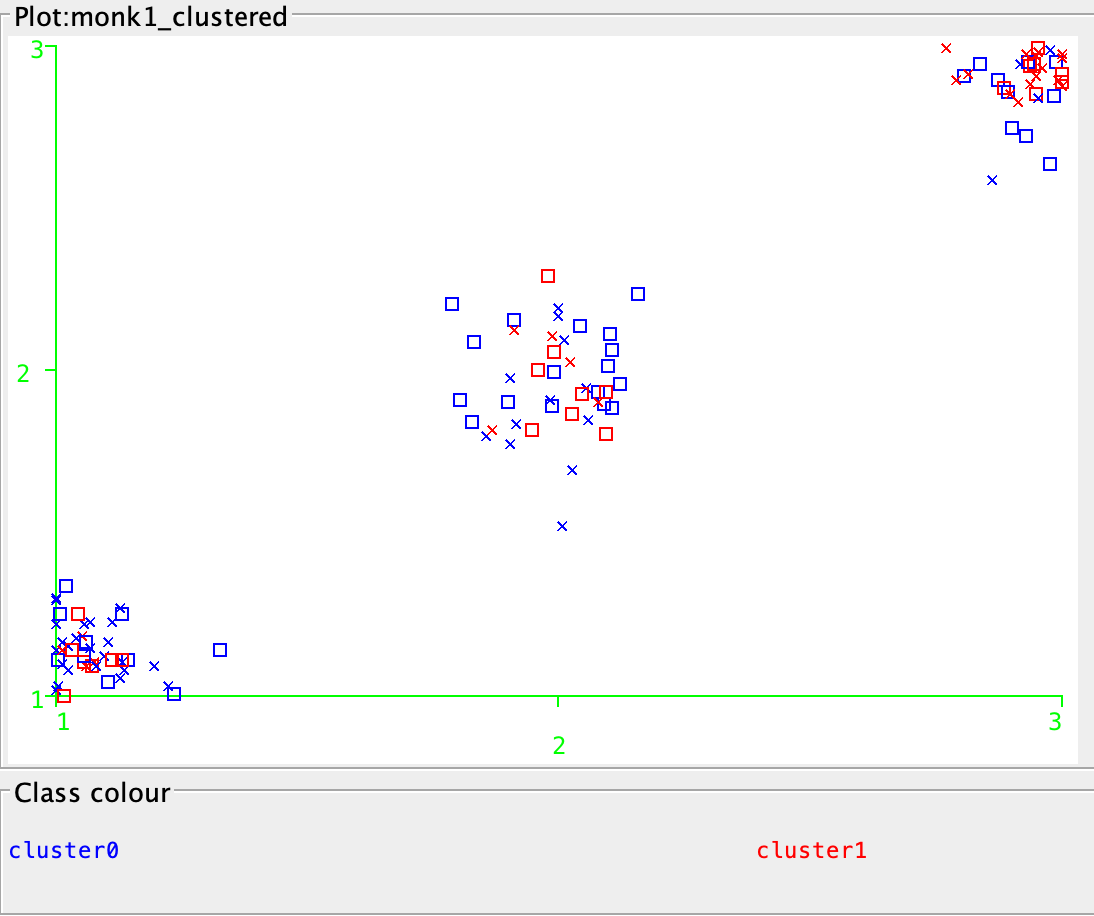
\includegraphics[width=70mm,scale=0.10]{Clustering_Visualization.png}
  \captionof{figure}{Overlapping data points}
\end{center}
\par
\textbf{Would you say that it goes poorly for monk1? Why or why not?} \par
From the data, we could conclude that the results of clustering algorithms were bad are because of
characteristics of the data. As said earlier, if we provide the preprocessed data to the algorithms,
we could get a better result and performance. But there is another way to handle this, i.e. we need 
to create a new distance function which can be incorporated into the existing algorithms to create
a separation for this type of data, but on the other hand, it requires lot of expertise and knowledge
for a domain for the data related to that domain.
\par
\textbf{\underline{Association Analysis}} \par
In order to perform association analysis on the dataset, it is not a thumb rule that similar points 
should lie close to each other, only rules are required to classify the points based on the pattern
in the data. \par

We then performed the \textbf{\textit{addCluster}} in the preprocess section and applied \textbf{\textit{Apriori 
Algorithm}}, and got the following association rules table which is given below; \par
\begin{center}
  \begin{tabular}{|c|c|c|c|}
    \hline
    \textbf{Association rule(s)} & \textbf{Cluster} & \textbf{Occurrence} & \textbf{Confidence} \\
    \hline
    attribute\#5=1 & 1 & 29 & 1 \\
    \hline
    attribute\#1=3 attribute\#2=3 & 1 & 17 & 1 \\
    \hline
    attribute\#5=1 attribute\#6=2 & 1 & 13 & 1 \\
    \hline
    attribute\#1=2 attribute\#2=2 & 1 & 15 & 1 \\
    \hline
  \end{tabular}
\end{center}
\par
We ignore some rules in the association analysis result where antecedent is a super set of antecedent of
another rule which are not useful for our analysis. Having lower confidence yields more information for
super set antecedent and we should not discard them. So, in this case the above rule of ignoring 
association rules where antecendent is a super set of antecendent of another rule applies, but it is not a
general rule, it can be applied when the rules have confidence = 1.
\end{document}